\documentclass[../SMLreport_template.tex]{subfiles}
 
\begin{document}
Boosting
Boosting is a type of sequential ensemble. The base model generated by each iteration mainly improves the place that the previous generation base model makes a mistake. It is an effective way to generate a strong learner by combined the weak learners. The weak learner is those algorithms that error rate is slightly below 50 $\%$, it is come from weak learning algorithm e.g. decision stump. Stump is a decision tree with just one node and two leaves. Therefore, it is suitable for high bias and low variance models.
There are two key question in boosting. How to change the weight of the training data in each iteration? How to combine the weak learner?
Boosting has a very powerful guarantee. If your algorithm can produce classifier with error rate smaller that 50 $\%$ on training data, then you can obtain 0 $\%$ error rate classifier after boosting.

AdaBoost
AdaBoost, short for adaptive boosting. It is the first adaptive algorithm, which can adapt to the respective training error rate of the weak learner. 
The motivation of the AdaBoost is even all weak classifier will make some immature decision, but the entire trained weak classifier will produce more accurate decisions. 

AdaBoost's process is following:
Given the same initial weight for each sample at beginning. After each round of weak learner training, the weight of each sample will be adjusted according to its performance. Increase the weight of misclassified sample and decrease the in the weight of correctly sample, so we can get more attention in the future. Each weak learner is made by considering previous weak learner’s mistakes.  According to this process, we repeatedly train M weak learners, and finally replace and combine them.
Figure 1
Before introducing the algorithm in detail, let's look at an example show in the figure 1. 
We have 10 sample points labeled + or -. Let 1 be + and 0 be -. Suppose our weak classifier is a horizontal or vertical line. It is easy to see that none of the lines can perfectly classify these 10 sample points. In first round, each sample have same weight, then we used the first weak classifier made by decision stump to classified. There are 3 sample points in the circle were misclassified. In second round we increase the weight of these 3 points and decrease the weight of other points. The result led by this action is we won’t make mistake in these 3 points, but it increases the probability other samples misclassified. Hence, we can create a new weak classifier which is much different than first weak learner. Same method in third round. We let first, second and third weak classifier be f1, f2 and f3 respective. Now we have 3 weak classifier and each of them have their own weight. The weight is calculated by adaboost formula which we have more detail in later section.

 
Figure 2

In the end, we combine the advantage of 3 weak classifier to generate a strong learner. As you can see, each weak classifier has 2 sections and it represents the two outcomes 1 and 0. After we combine the 3 weak classifiers, there are 6 sections and we need decide which outcome they belong to. For example, section b in the figure 3 is blue, this is because the weight of f1 and f2 is bigger than f2.

	Figure 3

AdaBoost's mathematical step:






















We use dataset ‘iris’ in R to show the advantages of ‘Adaboost’ Algorithm compared with other kinds of classification methods. In this part, R packages ‘Adabag’ is mainly used.\par
\subsection{Introduction to iris}
To aid this project, we need first to have a fundamental understanding of this dataset. ‘Iris’, which is initially collected by Fisher in 1936, is a widely used dataset for classification test around world. ‘Iris’ contains 150 samples with 3 categories and every sample has 4 attributes (Sepal Length; Sepal Width; Petal Length; Petal Width) and one specie. People make different classification function by this dataset and then try to predict what species some new samples (just have 4 attributes) might belong to.\par
\subsection{Applying Adaboost to ‘iris’}
\subsubsection{Making use of full data}
In this part, we do not consider train/test set. We use all of these 150 samples in ‘iris’ to show how Adaboost works. As decision tree is suitable for different types of parameters like numeric parameter, sequential parameter and so on, ‘boosting’ function in ‘adabag’ package uses decision tree which is also easily to choose parameters as the base classification (or weak learner). 
We use ‘boosting’ function to simulate the Adaboost algorithm and then make a prediction of species of these 150 samples. Finally, we calculate the error of our prediction to find out the accuracy of this model.\par
the confusion matrix is as follows:
 \begin{figure}[t]
    \centering
    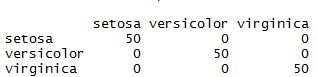
\includegraphics[width=0.5\textwidth]{sections/images/CM_of_full.jpg}
    \caption{Confusion matrix of full data}
\end{figure}
And it shows that the result of prediction is absolutely right and it seems that we get a good model from ‘adaboost’ in classification. 
Adaboost focus on data which is not predicted well in the last round, and then pay more attention to these samples in the next round, that means the model in the next step might perform better (smaller error). Thus, we get a chart that shows how errors change in different rounds.\par
 \begin{figure}[t]
    \centering
    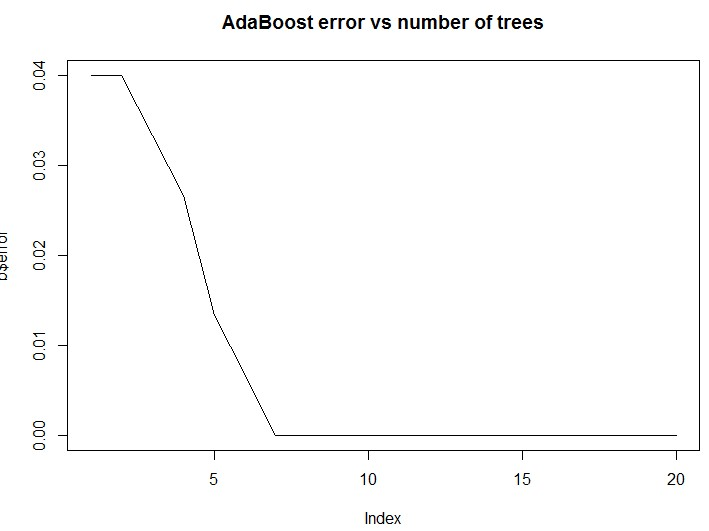
\includegraphics[width=0.5\textwidth]{sections/images/Errors.jpg}
    \caption{Errors in every step}
\end{figure}
It shows that error turn into 0 after 7 iterations, and we get a prediction error rate of zero.\par
As we have finished the adaboost algorithm, we could find how much every base classification weights. It shows that three base classifications have the highest weigths which is larger than 1.5 (number 8, 1, 19), On the other hand, base classification number 12 has the lowest weight (0.8403).\par
\begin{figure}[t]
    \centering
    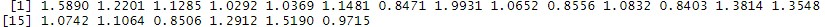
\includegraphics[width=0.5\textwidth]{sections/images/Weights_steps.jpg}
    \caption{Weights of every base classification}
\end{figure}

\subsubsection{Making use of partial data}
In this part, we take some random samples as train data and others as test data. We use train data to make a simulation and then make a prediction on the test data. At last we calculate the error to figure out whether the model is overfitting or not.\par

In every species we choose 40 samples and we get a train dataset of 120 samples in sum. We look over the results of both train data and test data and then calculate errors. Using the same function in the previous part and different data. 
The confusion matrixes are as follows,\par
 \begin{figure}[t]
    \centering
    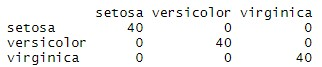
\includegraphics[width=0.5\textwidth]{sections/images/CM_of_train.jpg}
    \caption{Confusion matrix of train data}
\end{figure}

 \begin{figure}[t]
    \centering
    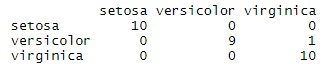
\includegraphics[width=0.5\textwidth]{sections/images/CM_of_test.jpg}
    \caption{Confusion matrix of test data}
\end{figure}
 
The results show that prediction in train set is 100 $\%$ right, while in test set, one virginica iris from the test data set were wrongly classified as versicolor class, so the error of test set reaches 3 $\%$. We can conclude that Adaboost on ‘iris’ is not overfitting.\par

\subsubsection{k-fold cross validation}
To avoid overfitting in Adaboost, we use k-fold cross validation. As dataset ‘iris’ only have 150 samples, it is very convenient and fast to do cross validation without dividing data set into training dataset and test dataset.\par

We apply 10-folds cross validation here and calculate the confusion matrix and error.
The results are as follows.\par
  \begin{figure}[t]
    \centering
    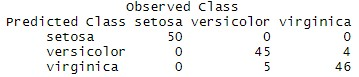
\includegraphics[width=0.5\textwidth]{sections/images/CM_of_10.jpg}
    \caption{Confusion matrix of 10-folds cross validation}
\end{figure}
It shows that in this case, there are 5 versicolor iris wrongly classified as virginica and 4 virginica iris wrongly classified as virginica. Thus, the error mean is 6 $\%$, which means that this model is not overfitting.

\end{document}